\begin{tcolorbox}
\chapter{2010 - Vodna Sled}

Vodna Sled 2010 was a clear success - in all we discovered 2.2 km of new
passage, all below -500 m, all in \passage{Vrtnarija} using \passage{Camp
X-Ray} (now a plush four bed camp at -550 m) as a base.

The major discovery was the swinging into the \passage{Leopard} lead from
\passage{Zimmer} chamber, leading to a 1.5 km complex of mainly horizontal
passage (\passage{Prince Consort Road}, \passage{Wonderland}), with many
unpushed leads for future years. Significant amounts of exploration also
took place in \passage{Tolminska Korita} concluding with a connection to
the deep level of \passage{Vrtnarija} (below \passage{Big Rock Candy Mountain}) at -653 m,
and pushing the \passage{Republika} streamway from -744 to -802 m.

A direct translation of "Vodna Sled" is difficult, but "Water Tracking / Following / Tracing" gives the general idea. This name was chosen as the all the leads in \passage{Vrtnarija} consisted of following streamways (\passage{Republica}, \passage{Fools / Falls Road}, \passage{Tolminska Korita}, \passage{Dangermouse}).


\end{tcolorbox}
\backgroundsetup{
    scale=1,
    color=black,
    opacity=1,
    angle=0,
    contents={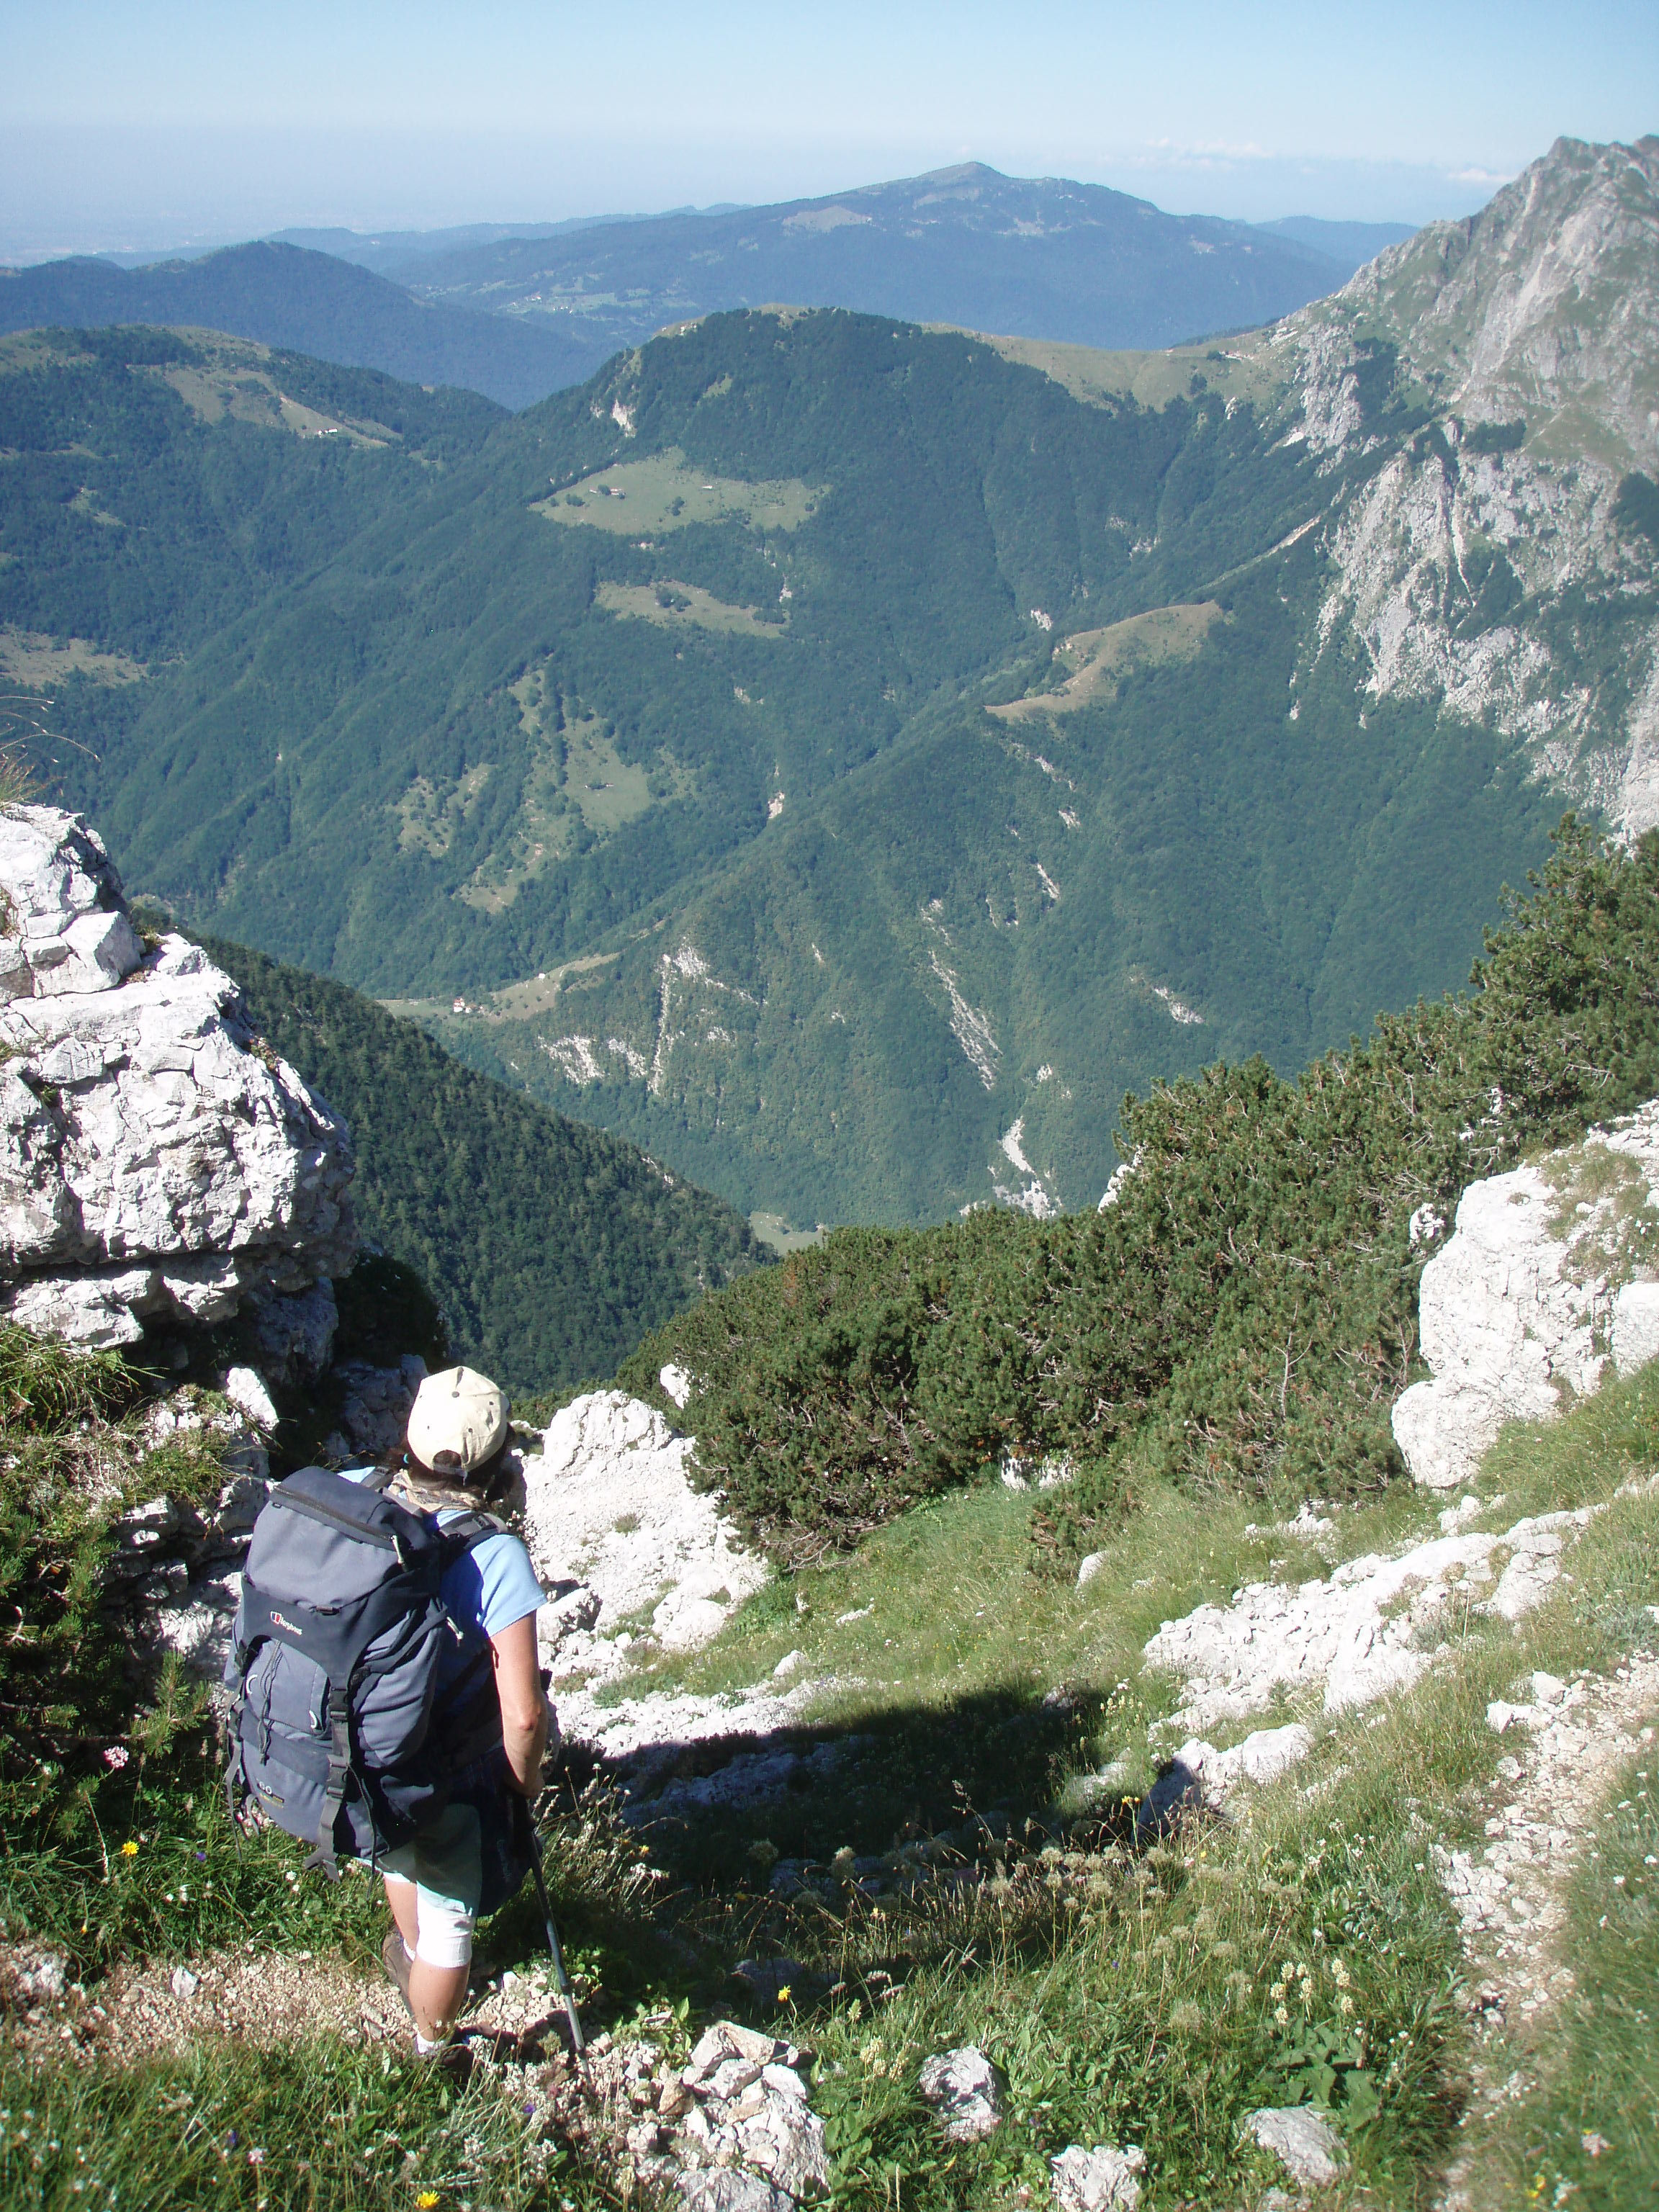
\includegraphics[height=\paperheight]{2010/intro/20100809-20-08-50 - Jan Evetts - P2090142 - Migovec Plateau--orig.jpg}}
}
\BgThispage









